\documentclass[preprint,12pt]{elsarticle}
\usepackage[T1]{fontenc}
\usepackage[utf8]{inputenc}
\usepackage{lmodern}
\usepackage{float,calc,amsmath,amssymb,booktabs,longtable,array,graphicx,pdflscape,xurl}
\usepackage[colorlinks=true,allcolors=blue]{hyperref}
\usepackage{microtype}
\usepackage{geometry}
\geometry{margin=24mm}
\usepackage{etoolbox,placeins}
\AtBeginEnvironment{longtable}{\scriptsize}
\setlength{\emergencystretch}{3em}
\providecommand{\tightlist}{\setlength{\itemsep}{0pt}\setlength{\parskip}{0pt}}
\providecommand{\pandocbounded}[1]{#1}
\makeatletter
\def\maxwidth{\ifdim\Gin@nat@width>\linewidth\linewidth\else\Gin@nat@width\fi}
\let\Oldincludegraphics\includegraphics
\renewcommand{\includegraphics}[2][]{\Oldincludegraphics[width=\maxwidth,#1]{#2}}
\makeatother
\hypersetup{pdfauthor={Alan Immanuel Benjamin Vallavaraj}}
\graphicspath{{../publishing/figures/}{./}}
\journal{Advanced Engineering Informatics}
\date{10 October 2026}
\begin{document}
\begin{frontmatter}
\title{Requirement-aware multi-lift dispatch: restricted waiting and accessibility trade-offs}
\author[westminster]{Alan Immanuel Benjamin Vallavaraj\corref{cor}}
\cortext[cor]{Corresponding author.}
\ead{a.vallavaraj@westminster.ac.uk}
\affiliation[westminster]{organization={School of Computer Science and Engineering, University of Westminster},addressline={115 New Cavendish Street},city={London},postcode={W1W 6UW},country={United Kingdom}}
\begin{abstract}
A lift-dispatch rule can shorten waits for passengers who request priority while lengthening waits for everyone else. This study represents occupancy, direction compatibility and priority requests as explicit dispatch, pickup and boarding rules, and evaluates them in a time-stepped simulator with a restricted mean waiting time that includes every arriving passenger, capped at 900 model time units. A 279,936-run historical campaign shows why this matters: a combined priority configuration has a 5.32\% completed-trip advantage, yet its general-request waiting does not improve, its completion is lower, and a sensitivity imputation for unserved passengers reverses the ranking. The primary evidence is a 16,848-run campaign on a corrected model, covering 108 building and demand scenarios with twelve matched arrival streams and 22,998,183 passenger records. It tests each priority component separately, adds door and transfer delays and varies the dispatch bonus. Priority-first boarding alone produces most of the priority benefit and of the cost to other passengers. With delays, full priority reduces priority-request waiting from 340.66 to 132.51 units relative to an occupancy-matched reference, while general-request waiting rises by 7.26 units (95\% paired scenario-bootstrap interval 5.34 to 9.40). Overall capped waiting falls by 8.68 units, but intervals for horizon-accrued waiting and overall completion include zero. Against collective dispatch, general-request waiting falls instead, so the baseline determines the apparent cost. Bonuses of $-1.4$, $-2.8$ and $-4.2$ give closely similar outcomes, and the trade-off holds at horizons from 300 to 1,200 units. The results quantify a service-allocation choice rather than general controller superiority.
\end{abstract}
\begin{keyword}lift group control \sep priority requests \sep knowledge representation \sep restricted waiting \sep simulation \sep reproducibility\end{keyword}
\end{frontmatter}
\section{Introduction}\label{introduction}

A lift can arrive promptly and still provide poor service if the car has insufficient space to board waiting passengers. Priority boarding introduces a second question: how should a group of cars serve an explicitly prioritised request while maintaining reasonable service for the remaining passengers? A building-wide average can conceal both an unequal allocation of waiting time and passengers who never board during the observation period.

Occupancy-aware group dispatch, traffic-aware learning and priority scheduling have already been studied in engineering informatics \cite{ref1,ref3,ref5}. Occupancy sensing, coordinated dispatch and accessibility priority are therefore not claimed as new concepts here. The question is narrower: what service trade-offs arise when occupancy and priority requirements are represented by explicit rules, and do the conclusions survive an evaluation that includes every arriving passenger?

The study uses two campaigns. A 279,936-run historical factorial campaign shows how completed-trip means can misstate the effect of a priority rule when completion differs between configurations. A 16,848-run campaign on a corrected model, with matched arrival streams and complete passenger-event records, provides the primary evidence. It separates the priority rule into its components, adds door and transfer delays, varies the dispatch bonus and evaluates every arrival over a common horizon. An intermediate event-recording campaign on the legacy model is superseded by the corrected campaign and reported in \ref{app:legacy}.

The study makes three contributions. First, it maps passenger and car facts explicitly to dispatch, pickup and boarding rules (Table~\ref{tab:rules} and Eqs.~\eqref{eq:score}--\eqref{eq:boarding}), so that each service requirement can be traced to a rule and to the outcome used to evaluate it. Second, it evaluates those rules with a restricted mean waiting time that includes unboarded passengers and is reported separately for priority and general requests, and it shows how completed-trip means can misstate the result. Third, matched-arrival ablation, delay and bonus experiments locate the source of the priority benefit and quantify who bears its cost, with paired scenario-bootstrap intervals. No learning algorithm or physical ride-comfort controller is proposed.

\section{Related work}\label{related-work}

\subsection{Lift group control and passenger information}\label{lift-group-control-and-passenger-information}

Wang et al.~use occupancy information and usage-pattern learning to support lift group control \cite{ref1}. Wan et al.~address traffic-aware dispatch with reinforcement learning \cite{ref3}. Han et al.~investigate priority scheduling using image analytics for passengers requiring priority access \cite{ref5}. These are the closest application precedents. The present study does not reimplement their complete systems.

Earlier dispatch approaches include fuzzy control \cite{ref11,ref16,ref25}, heuristic search \cite{ref12}, genetic and tabu search \cite{ref13,ref15}, multi-agent reinforcement learning \cite{ref26} and combinatorial optimisation \cite{ref28}. Double-deck systems introduce further installation-specific decisions \cite{ref24}. These studies motivate comparing decision rules within a shared environment, while recognising that a simplified comparator does not stand in for an independently validated industrial controller.

Camera-assisted group control and passenger detection have also been investigated \cite{ref17,ref20,ref21}. Occupancy tracking in buildings \cite{ref19} and thermal-camera assessment of occupant comfort \cite{ref18} concern distinct measurements. They do not justify inferring a passenger's accessibility requirements or stability from appearance. In the present experiments, a priority request is a supplied binary input, not the output of a camera or a diagnosis.

\subsection{Representation and evaluation}\label{representation-and-evaluation}

Occupant-presence models \cite{ref14}, uncertain passenger-arrival formulations \cite{ref27} and independently developed lift simulators \cite{ref22,ref23,ref29} show that performance depends on the demand and movement models. Digital-twin architectures \cite{ref30,ref31} provide context for linking observations and decisions, but an offline time-stepped simulation is not a deployed digital twin.

Scheduling frameworks for automated storage yards \cite{ref2}, shared manufacturing \cite{ref4} and cloud--edge production \cite{ref10} keep the state representation, the decision mechanism and the evaluation distinct. Human-centred decision studies make the same separation for people's requirements: preference-aware task allocation \cite{ref7}, context-aware motion prediction \cite{ref8}, knowledge-integrated assembly planning \cite{ref9}, ergonomic role allocation \cite{ref32} and evacuation-choice modelling \cite{ref6} each treat human requirements as declared inputs whose effects are evaluated separately. Here the representation is a small set of explicit facts and rules rather than a learned policy, ontology reasoner or general-purpose knowledge graph. Its purpose is traceability: each requirement maps to an action and to the outcome used to judge it.

\subsection{Observation horizons and the research question}\label{observation-horizons-and-the-research-question}

Completed-trip waiting is conditional on reaching the destination before observation ends, and this condition can differ between controllers. A lower conditional mean can coexist with more unserved passengers, so it cannot alone identify a population-wide service gain. The present study therefore evaluates a restricted mean waiting time from arrival to boarding over all generated passengers, the waiting analogue of the restricted mean survival time used for censored time-to-event outcomes \cite{refRMST}. It reports destination completion separately and distinguishes group means from averages of within-run ratios.

\section{Requirement representation and dispatch rules}\label{requirement-representation-and-dispatch-rules}

\subsection{State and requirements}\label{state-and-requirements}

At time $t$, car $c$ is represented by its floor $x_c$, direction $d_c\in\{-1,0,1\}$, capacity $C$, onboard passenger set, and target floors. Its load ratio is $\rho_c=n_c/C$, where $n_c$ is the number of passengers on board. A request contains an arrival time, origin, destination and priority indicator $p_i\in\{0,1\}$. The priority indicator represents an externally supplied request for prioritised service. It does not represent a diagnosis, impairment severity or an inferred instability risk.

Table~\ref{tab:rules} links the state facts to rule actions and to the outcome used to evaluate each requirement. Capacity is a count of $C=13$ passengers per car. Neither passenger mass nor the spatial footprint of mobility aids is represented, so an occupancy ratio is a passenger-count ratio and cannot establish that a car has sufficient accessible floor space in a real installation.

\begin{longtable}{@{}p{.22\linewidth}p{.21\linewidth}p{.30\linewidth}p{.19\linewidth}@{}}
\caption{Requirement facts, rule actions and evaluation outcomes.}\label{tab:rules}\\
\toprule Requirement & Facts used & Rule action & Evaluation outcome\\\midrule\endhead
\bottomrule\endlastfoot
Reach a waiting request & Car floor; request floor & Minimise distance, with a direction term (Eq.~\eqref{eq:score}) & Restricted wait\\
Account for occupied capacity & Passenger count; capacity & Load penalty (Eq.~\eqref{eq:score}); pickup gate (Eq.~\eqref{eq:pickup}) & Boarding and completion\\
Prioritise a supplied request & Priority flag; remaining capacity & Dispatch bonus (Eq.~\eqref{eq:score}), pickup exception (Eq.~\eqref{eq:pickup}) and priority-first boarding (Eq.~\eqref{eq:boarding}) & Priority-group restricted wait\\
Preserve service for other requests & Arrival order; direction & Arrival-order boarding within groups, with direction compatibility (Eq.~\eqref{eq:boarding}) & General-group restricted wait\\
\end{longtable}

\subsection{Assignment and pickup}\label{assignment-and-pickup}

Every eight time steps, each floor $f$ with a non-empty queue $Q_f$ is assigned a car. Let $\delta_f$ be the majority direction of the queue and $\pi_f=1$ if any request in $Q_f$ has $p_i=1$. Four binary flags describe a configuration: the occupancy rules $O$, the priority dispatch bonus $D$, priority-first boarding $B$ and the priority pickup exception $E$. The assigned car minimises
\begin{equation}
\begin{split}
s_c(f,t) ={}& |x_c-f| + 2.5\,\mathbf{1}[d_c\neq 0,\ \delta_f\neq 0,\ d_c\neq\delta_f] + 10\,O\,\max(0,\rho_c-0.78)\\
&- \beta\,D\,\pi_f\,(1-\rho_c) + \varepsilon(f,t,c),
\end{split}
\label{eq:score}
\end{equation}
where $\beta=2.8$ unless stated otherwise and $\varepsilon\in[0,0.02)$ breaks ties. The collective reference is the configuration with all four flags off.

When a car reaches an assigned floor, the pickup gate decides whether it opens for the waiting queue. With $n'_c$ passengers remaining after alighting, $\rho'_c=n'_c/C$ and queue length $q_f$, occupancy configurations ($O=1$) apply, in order,
\begin{equation}
G_c(f)=\begin{cases}
0 & \text{if } \rho'_c\ge 0.92 \text{ and not } \bigl(E\,\pi_f=1 \text{ and } n'_c<C\bigr),\\
E\,\pi_f & \text{otherwise, if } \rho'_c\ge 0.82 \text{ and } q_f>\max(1,\,C-n'_c),\\
1 & \text{otherwise},
\end{cases}
\label{eq:pickup}
\end{equation}
and $G_c(f)=1$ when $O=0$. The thresholds are fixed and were not tuned using the reported outcomes.

The distance-only nearest-car reference selects the car with minimum $|x_c-f|$, breaking equal distances by car identifier. It has no direction, occupancy or priority term and boards in arrival order. It is an explicitly specified conventional reference rule, not a reproduction of a complete published nearest-car implementation, and it differs from the historical configuration named nearest\_car, which uses the same decision logic as the historical collective configuration.

\subsection{Boarding, movement and delays}\label{boarding-and-movement}

Boarding orders the queue lexicographically by
\begin{equation}
k_i=\bigl(B\,(1-p_i),\ a_i,\ i\bigr),
\label{eq:boarding}
\end{equation}
so that, when $B=1$, priority requests board first and each group boards in arrival order $a_i$. Passengers are admitted in this order until the car is full. When the car still carries passengers after alighting, a passenger whose direction differs from the car's travel direction (or, for an idle car, from the queue's majority direction) is skipped.

Cars move one floor per model time step towards their targets, continuing while targets remain ahead and reversing otherwise. A stationary car heads for its nearest target. Equidistant targets are resolved by the iteration order of the target set, a detail that matters for exact replay (\ref{app:legacy}).

Without delays, transfers occur at the stop and the car moves in the same step. In the delay configurations, a stop incurs five fixed model time units, then one unit for each alighting passenger and then one for each boarding passenger. Transfers are recorded at completion, physical occupancy changes at each transfer and the car cannot move during service. Boarding reserves a cohort using the capacity left after planned alighting, and later arrivals wait for another service cycle. No busy-time term is added to Eq.~\eqref{eq:score}. The delay values are simple assumptions, not calibrated operational measurements.

These abstractions support a comparison of rules within the model; they are not calibrated predictions for a building. No speed adaptation, acceleration, physical jerk or measured energy model is evaluated. The synthetic stability, comfort and guidance accounting of the historical simulator is not part of the corrected model and is not used as an outcome.

\section{Experimental design and outcomes}\label{experimental-design-and-outcomes}

\subsection{Historical factorial campaign}\label{historical-factorial-campaign}

Table~\ref{tab:historical} summarises the historical campaign. Seven factors give 2,916 combinations, which with eight configurations and twelve seeds give 279,936 runs. Each run generates Poisson arrivals with traffic-dependent intensity for 3,600 steps and allows up to 900 clearance steps. The historical simulator is the legacy model: it predates the corrections of Section~\ref{sec:design} and uses no door or transfer delay.

\begin{longtable}{@{}p{.36\linewidth}p{.56\linewidth}@{}}
\caption{Historical factorial design.}\label{tab:historical}\\
\toprule Factor & Levels\\\midrule\endhead
\bottomrule\endlastfoot
Floors & 8, 16, 32\\
Cars & 2, 4, 8\\
Population scale & 200, 800, 2,000\\
Traffic & Up-peak, down-peak, lunch, mixed\\
Priority-request share & 0.02, 0.08, 0.15\\
Carrying-object share & 0.05, 0.20, 0.40\\
Synthetic noise & 0.00, 0.08, 0.18\\
Configurations and seeds & Eight historical configurations; seeds 0--11\\
\end{longtable}

The historical outputs contain run-level means and counts, not individual waiting or censoring times. Conditional mean waiting and completion can be reconstructed, but a passenger-level restricted mean cannot be recovered from those summaries. The campaign is therefore used only to show how completed-trip means behave (Section~\ref{sec:historical-results}). Its exposure, noise and guidance outputs are not outcomes. The full experiment history is listed in Table~\ref{tab:history}.

\subsection{Corrected matched-arrival campaign}\label{sec:design}

The primary evidence comes from a bounded campaign on a corrected model version (Table~\ref{tab:design}). The diagonal floor/car pairs (8, 2), (16, 4) and (32, 8) are crossed with three population scales, four traffic patterns and three priority-request shares, giving 108 structural scenarios, each run with twelve seeds. Thirteen configurations share identical arrival records within each scenario--seed pair. This was verified with a hash of passenger identifier, origin, destination, arrival time and synthetic attributes.

\begin{table}[htbp]\centering
\caption{Design of the corrected matched-arrival campaign.}\label{tab:design}
\small\begin{tabular}{@{}p{.28\linewidth}p{.66\linewidth}@{}}
\toprule Design element & Value\\\midrule
Structural scenarios & Floor/car pairs (8, 2), (16, 4), (32, 8) $\times$ population 200, 800, 2,000 $\times$ four traffic patterns $\times$ priority share 0.02, 0.08, 0.15 $=108$\\
Fixed factors & Carrying share 0.20 and synthetic noise 0.08; neither enters the corrected model's decisions\\
Configurations without delay & Occupancy reference; dispatch only; boarding only; pickup exception only; full priority ($\beta=2.8$); full priority with $\beta=1.4$ and $\beta=4.2$; collective; distance-only nearest car\\
Configurations with delay & Occupancy reference, full priority, collective and distance-only nearest car, each with five fixed units per stop and one unit per transfer\\
Replications & Twelve seeds; identical arrival streams across all thirteen configurations\\
Horizons & Arrivals 0--3,599; observation to $T=4{,}500$; restricted horizon 900 (sensitivity 300--1,200)\\
Runs and records & 16,848 runs, of which 5,184 with delays; 22,998,183 passenger records\\
Execution & Python 3.12.1 and NumPy 2.3.5; source files and protocol fixed and hashed before execution\\
\bottomrule
\end{tabular}
\end{table}

Nine configurations have no door or transfer delay. Five of them form the ablation: an occupancy reference with $O=1$ and no priority component, the dispatch bonus alone ($D=1$), priority-first boarding alone ($B=1$), the pickup exception alone ($E=1$), and the full priority rule ($D=B=E=1$). Holding the occupancy penalty and pickup gate fixed in all five arms makes the contribution of each component, including the exception, interpretable. Two further full-rule arms use $\beta=1.4$ and $\beta=4.2$, and collective dispatch ($O=0$) and the distance-only nearest car complete the set. Four configurations repeat the occupancy reference, full priority, collective and distance-only arms with the delay model of Section~\ref{boarding-and-movement}.

Two corrections distinguish this model from the legacy simulator, and both apply to every configuration. First, a served or empty target floor is removed when a car stops; the legacy simulator could retain such stale targets and travel to them unnecessarily. Second, the tie-break term $\varepsilon$ in Eq.~\eqref{eq:score} is a counter-based pseudorandom value keyed by seed, time, calling floor and car, so every configuration sees the same values; the legacy simulator drew it from a configuration-specific random stream shared with unused comfort accounting. Contrasts are therefore computed only within the corrected model. An earlier 5,184-run event-recording campaign on the legacy simulator is superseded by this campaign and reported in \ref{app:legacy}.

The grid, configurations and analysis were fixed in a protocol before execution. Six invariant checks and a 26-case development smoke test preceded the run, and the stopping rule permitted only recovery of technically missing cases. No case was excluded or repeated on the basis of performance. Every run's passenger events were reconstructed and checked against its summary, including cohort hashes, group counts, transfer order and restricted waiting.

\subsection{Restricted mean waiting time}\label{fully-observed-restricted-waiting}

For passenger $i$ with arrival time $a_i$ and boarding time $b_i$, observed until $T=4{,}500$, the waiting time and its restricted mean over a set of passengers $P$ are
\begin{equation}
W_i=\begin{cases} b_i-a_i & \text{if } i \text{ boards before } T,\\ T-a_i & \text{otherwise},\end{cases}
\qquad
R_h(P)=\frac{1}{|P|}\sum_{i\in P}\min(W_i,h).
\label{eq:restricted}
\end{equation}
Every arrival occurs by time 3,599, so $T-a_i\ge 901$ and $R_h$ is fully observed for every passenger whenever $h\le 900$. The primary outcome is $R_{900}$, computed for all, priority and general requests within each run and then averaged with equal weight across runs. A boarded passenger counts as served even if alighting is not complete.

Destination completion and horizon-accrued waiting, the uncapped mean of $W_i$, are secondary outcomes. Horizon-accrued waiting is a finite-horizon service burden, not an estimate of eventual waiting beyond observation. The horizon sensitivity recomputes $R_h$ from the retained passenger events at $h=300$, 600 and 900, all fully observed, and at $h=1{,}200$ over the 93.81\% of arrivals with at least 1,200 units of follow-up.

\subsection{Paired uncertainty and fairness}\label{paired-uncertainty-and-fairness}

For the corrected campaign, intervals resample the 108 structural scenarios with all twelve seeds and all configurations kept together, so every contrast is paired. For the historical campaign, they resample 972 structural blocks defined by floors, cars, population, traffic, priority share and carrying share, keeping all three noise levels and twelve seeds together so that invariant noise replicates are not treated as independent evidence. Both use 2,000 bootstrap draws with seed 20261008 and percentile 95\% intervals, without multiplicity correction.

The intervals describe variation over the fixed design-scenario composition. The scenarios are not a random sample of real buildings, and the intervals do not quantify model calibration uncertainty. Run-level means receive equal weight. Historical completion fractions are passenger-weighted; corrected-campaign completion is an average of run-level fractions.

The archived fairness\_disparity field is an average of run-level priority/general waiting ratios with a denominator floor of one, not the ratio of the two aggregate group means, and low general-group waits make it unstable. Each group's wait is therefore reported directly, with ratios of aggregate group means as a separate descriptive quantity. Neither ratio alone defines an appropriate allocation of service.

\section{Results}\label{results}

\subsection{Completed-trip means in the historical campaign}\label{sec:historical-results}

Table~\ref{tab:conditional} presents the principal historical configurations. The historical layered configuration, which added a stability-related dispatch penalty and synthetic exposure accounting to the priority rule, has a conditional mean waiting time of 349.87 units against 369.54 for the collective reference, a reduction of 5.32\% (clustered interval 4.10\% to 6.56\%). The apparent overall gain is carried by priority requests. The layered configuration's general-request wait is 372.40 against 370.81, a paired difference of 1.59 units ($[-8.16, 10.00]$), and its passenger-weighted completion is lower, at 74.45\% against 75.97\% (Figure~\ref{fig:conditional}).

\begin{longtable}{@{}p{.28\linewidth}rrrr@{}}
\caption{Historical completed-trip-only waits and passenger-weighted completion.}\label{tab:conditional}\\
\toprule Configuration & Conditional wait & Priority wait & General wait & Completion (\%)\\\midrule\endhead
\bottomrule\endlastfoot
Priority rule & 350.44 & 129.41 & 373.66 & 74.61\\
Collective reference & 369.54 & 353.46 & 370.81 & 75.97\\
Historical layered & 349.87 & 133.19 & 372.40 & 74.45\\
Occupancy rule & 377.12 & 358.40 & 378.49 & 74.84\\
\end{longtable}

\begin{figure}[H]\centering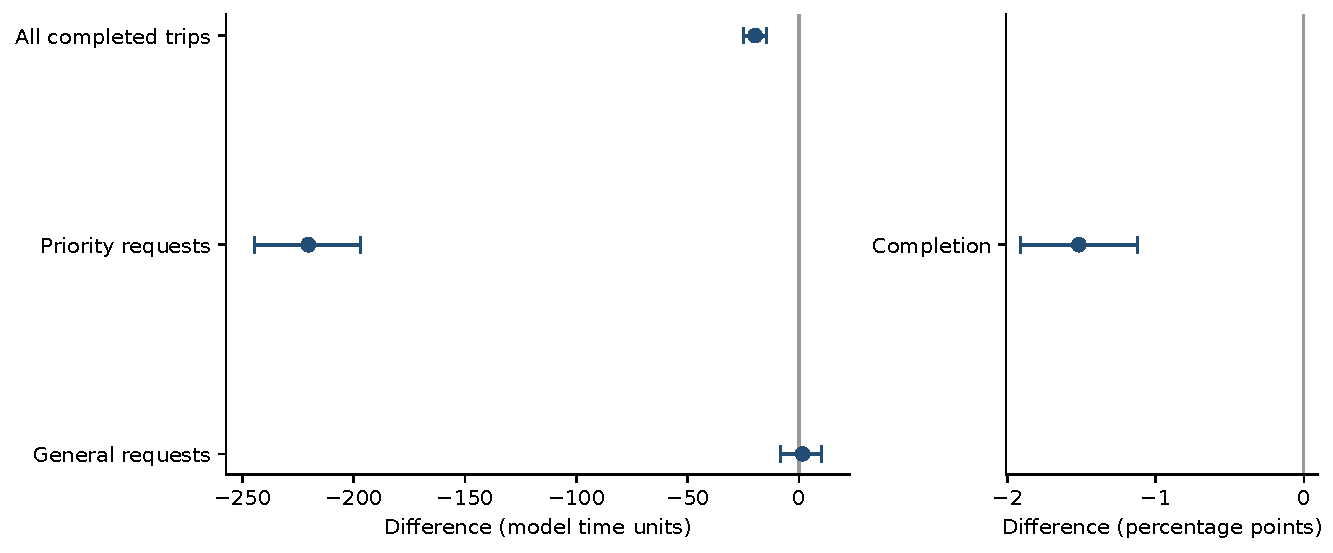
\includegraphics[width=\linewidth]{conditional_contrasts.pdf}
\caption{Historical layered configuration versus the collective reference. Points are paired differences in completed-trip group means and in passenger-weighted completion; bars are 95\% structural-scenario bootstrap intervals. These conditional differences do not establish an improvement over all arrivals.}\label{fig:conditional}\end{figure}

Because completion differs, the conditional means describe different passenger populations. Without individual observation times, the historical CSV bounds the finite-horizon waiting burden only broadly. For the layered configuration, the completed-trip contribution per generated passenger is 190.43 units, and adding the maximum possible accrued wait for unresolved passengers gives an upper bound of 1,339.76; the corresponding range for the reference is 203.92 to 1,284.97. The ranges overlap, so the data cannot determine which configuration has lower all-arrival waiting. As a sensitivity calculation rather than recovered data, assigning every unresolved passenger 1,000 units gives 445.89 for the layered configuration and 444.21 for the reference, reversing the ordering of passenger-weighted conditional waiting. This is a different aggregation from the 5.32\% run-mean comparison and is not a corrected version of that percentage.

The two fairness summaries also point in opposite directions. The archived mean of run-level ratios rises from 1.00 to 2.48 for the layered configuration, while the ratio of aggregate priority to general means falls from 0.95 to 0.36. The difference arises from the aggregation operations and small denominators, so neither should be read as a measure of improved or worsened fairness. These limitations motivate the restricted mean over all arrivals used in the rest of this section.

\subsection{Component ablation}\label{sec:ablation}

Table~\ref{tab:ablation} reports the corrected campaign without delays. Priority-first boarding reproduced most of the full rule's priority benefit (Figure~\ref{fig:ablation}). Relative to the occupancy reference, boarding alone reduced priority restricted waiting by 165.13 units ($[-209.61,-124.04]$) while increasing general-request waiting by 6.26 units ($[4.56,8.20]$). The corresponding full-rule differences were $-165.55$ ($[-209.95,-124.46]$) and $+6.08$ ($[4.27,8.03]$). Dispatch alone changed priority waiting by $-0.02$ units ($[-0.51,0.47]$), and the pickup exception alone by $-0.24$ ($[-0.48,-0.06]$). Boarding alone is therefore sufficient to produce most of the effect in this design; the singleton arms do not show that it is necessary or resolve every interaction among components.

\begin{longtable}{@{}p{.30\linewidth}rrrr@{}}
\caption{Corrected-model outcomes without delays. Waiting is restricted to 900 model time units and averaged over all 1,296 runs per configuration.}\label{tab:ablation}\\
\toprule Configuration & All & Priority & General & Completion (\%)\\\midrule\endhead
\bottomrule\endlastfoot
Occupancy reference & 203.96 & 200.78 & 204.24 & 88.04\\
Dispatch only & 203.90 & 200.76 & 204.19 & 88.04\\
Boarding only & 196.81 & 35.65 & 210.50 & 88.06\\
Pickup exception only & 203.80 & 200.54 & 204.09 & 88.04\\
Full priority & 196.64 & 35.22 & 210.33 & 88.05\\
Collective & 205.38 & 202.09 & 205.67 & 88.02\\
Distance-only nearest car & 226.12 & 222.42 & 226.41 & 87.09\\
\end{longtable}

\begin{figure}[H]\centering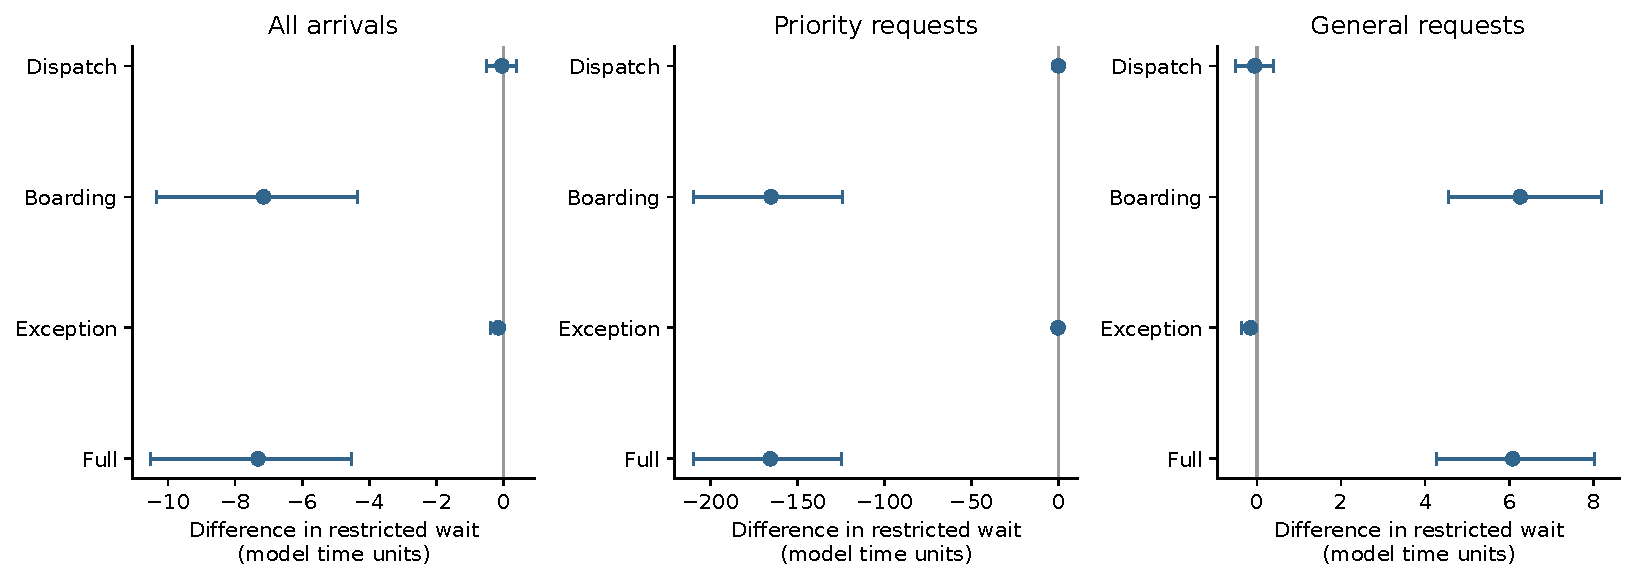
\includegraphics[width=\linewidth]{aei_ablation.pdf}
\caption{Component effects relative to the occupancy-matched reference, without delays. Points show paired differences in 900-unit restricted waiting; horizontal bars show 95\% scenario-bootstrap intervals. Negative values indicate lower waiting, and each panel uses its own scale. Boarding alone yields most of the priority benefit and of the general-request cost; singleton arms do not constitute a complete factorial interaction analysis.}\label{fig:ablation}\end{figure}

The full rule reduced overall restricted waiting by 7.31 units relative to the occupancy reference ($[-10.52,-4.54]$), but changed horizon-accrued waiting by only $+0.36$ ($[-0.53,1.27]$) and overall completion by $+0.016$ percentage points ($[-0.009,0.043]$). Priority completion rose by 11.72 percentage points and general completion fell by 1.10 points. A lower capped mean therefore does not imply better eventual service or higher total throughput. Against collective dispatch, overall restricted waiting fell by 8.73 units ($[-12.01,-5.73]$), while general-request waiting rose by 4.66 ($[1.95,7.27]$).

\subsection{Door and transfer delays}\label{sec:dwell}

Introducing door and transfer delays increased absolute waiting markedly: collective restricted waiting rose from 205.38 to 357.14 units. The 5,184 runs with delays retained the direction of the priority effect (Table~\ref{tab:dwell}, Figure~\ref{fig:dwell}). Relative to the occupancy reference, full priority reduced priority waiting from 340.66 to 132.51 units, a difference of $-208.15$ ($[-247.76,-170.90]$), or 61.10\%. General waiting rose from 344.38 to 351.64, a difference of $+7.26$ ($[5.34,9.40]$). Overall restricted waiting fell by 8.68 units ($[-11.50,-5.93]$), while the horizon-accrued difference was $-0.84$ ($[-2.51,0.78]$). General completion fell by 1.55 percentage points ($[-2.07,-1.07]$), and the interval for overall completion included zero.

\begin{longtable}{@{}p{.30\linewidth}rrrr@{}}
\caption{Corrected-model outcomes with five fixed units per stop and one unit per passenger transfer; 1,296 runs per configuration.}\label{tab:dwell}\\
\toprule Configuration & All & Priority & General & Completion (\%)\\\midrule\endhead
\bottomrule\endlastfoot
Occupancy reference & 344.08 & 340.66 & 344.38 & 79.60\\
Full priority & 335.40 & 132.51 & 351.64 & 79.63\\
Collective & 357.14 & 353.40 & 357.48 & 78.30\\
Distance-only nearest car & 363.57 & 359.42 & 363.94 & 78.10\\
\end{longtable}

\begin{figure}[H]\centering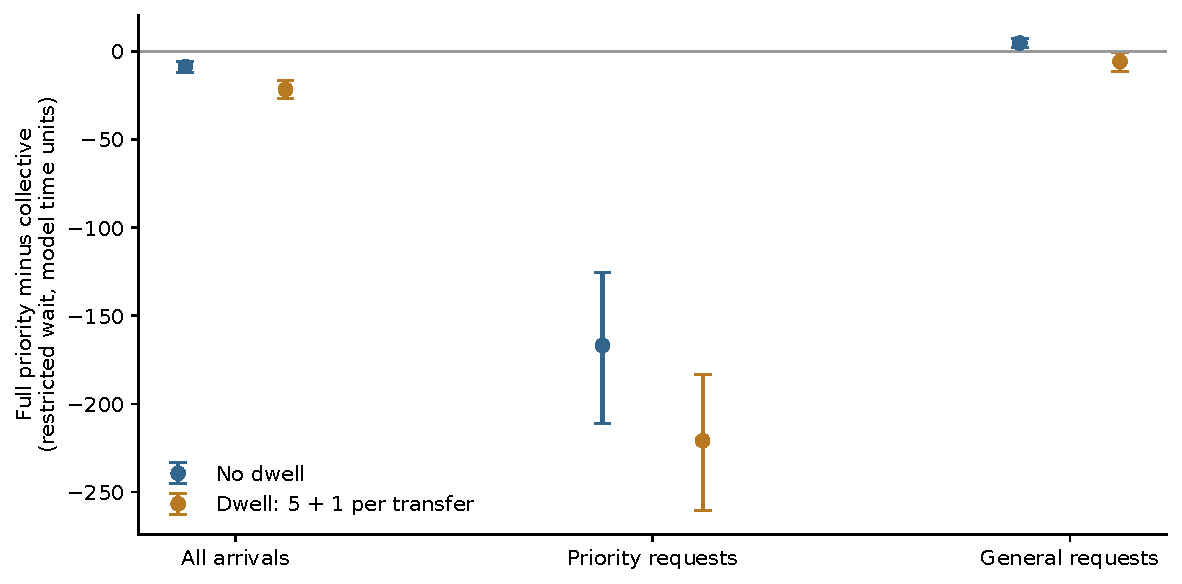
\includegraphics[width=.82\linewidth]{aei_dwell.pdf}
\caption{Full priority versus collective dispatch without delays and with five fixed units per stop plus one per transfer. Points are paired differences in 900-unit restricted waiting and bars are 95\% scenario-bootstrap intervals, for all, priority and general arrivals. With delays the general-request comparison against collective dispatch changes sign, unlike the general-request cost relative to the occupancy reference (Table~\ref{tab:dwell}).}\label{fig:dwell}\end{figure}

The choice of baseline determines the apparent cost. With delays, full priority also reduced general waiting relative to collective dispatch, by 5.84 units ($[-11.49,-0.74]$), and reduced overall waiting by 21.74 ($[-26.81,-16.82]$). Overall completion rose by 1.33 percentage points ($[0.64,2.14]$), whereas the general completion difference of $-0.25$ points had an interval spanning zero. These combined-rule comparisons do not isolate priority: under delays, the occupancy rules alone reduce general waiting by about 13 units relative to collective dispatch (344.38 against 357.48 in Table~\ref{tab:dwell}), which more than offsets the cost of priority. The occupancy-matched comparison isolates the general-request cost.

\subsection{Priority bonus sensitivity}\label{sec:weights}

All three bonuses produced closely similar restricted waiting (Table~\ref{tab:weights}, Figure~\ref{fig:weights}). Compared with $\beta=2.8$, using $\beta=1.4$ changed priority waiting by $+0.05$ units ($[-0.11,0.24]$) and using $\beta=4.2$ changed it by $-0.11$ ($[-0.34,0.12]$). The corresponding general-request changes were $+0.09$ ($[-0.01,0.22]$) and $-0.03$ ($[-0.14,0.09]$). When priority-first boarding is enabled, the outcome is insensitive to the dispatch bonus within this range. This is bounded evidence, not proof of equivalence outside the tested range, and no bonus was selected after inspecting outcomes.

\begin{longtable}{@{}p{.30\linewidth}rrrr@{}}
\caption{Bonus sensitivity with all three priority components enabled and no delays.}\label{tab:weights}\\
\toprule Configuration & All & Priority & General & Completion (\%)\\\midrule\endhead
\bottomrule\endlastfoot
Full priority, $\beta=1.4$ & 196.72 & 35.28 & 210.42 & 88.05\\
Full priority, $\beta=2.8$ & 196.64 & 35.22 & 210.33 & 88.05\\
Full priority, $\beta=4.2$ & 196.61 & 35.12 & 210.30 & 88.05\\
\end{longtable}

\begin{figure}[H]\centering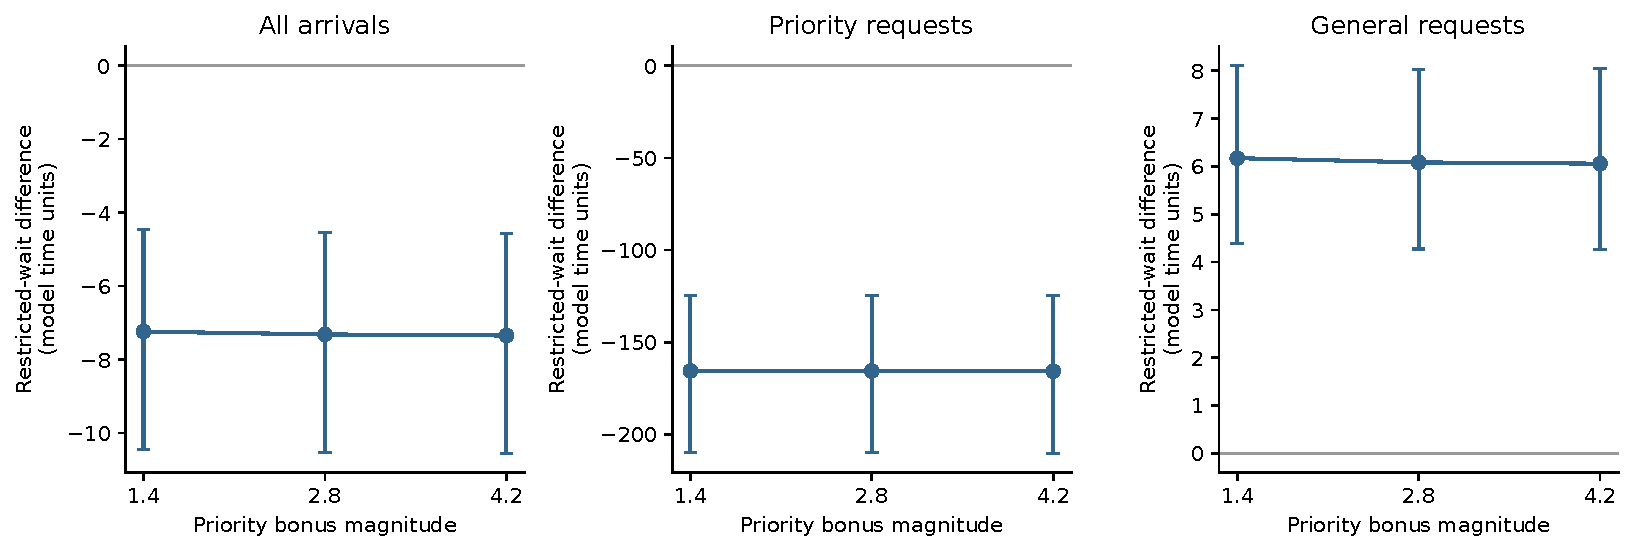
\includegraphics[width=\linewidth]{aei_weights.pdf}
\caption{Restricted-wait differences relative to the occupancy reference at bonus magnitudes $\beta=1.4$, 2.8 and 4.2, with all priority components enabled and no delays. Bars show 95\% scenario-bootstrap intervals. Direct paired intervals for the change between bonus values are reported in Section~\ref{sec:weights}.}\label{fig:weights}\end{figure}

\subsection{Restricted-horizon sensitivity}\label{restricted-horizon-sensitivity}

Table~\ref{tab:horizon-sensitivity} recomputes the occupancy-matched contrasts at four horizons from the retained passenger events; the 900-unit values reproduce Sections~\ref{sec:ablation} and~\ref{sec:dwell} exactly. At every horizon, with and without delays, full priority lowers priority-request waiting, raises general-request waiting and lowers the capped overall mean, and no interval includes zero. Both the benefit and the cost grow with the horizon, because a longer cap counts more of the longest waits. Against collective dispatch without delays, the general-request difference is small at short horizons and its interval includes zero at 300 and 600 units ($0.41$, $[-1.01,1.56]$; $2.12$, $[-0.07,3.98]$). With delays it remains negative except at 1,200 units, where the interval includes zero ($-4.74$, $[-11.71,1.53]$). The service-allocation conclusion therefore does not depend on the choice of a 900-unit horizon.

\begin{table}[htbp]\centering
\caption{Full priority minus the occupancy reference in restricted waiting at four horizons; positive values indicate longer waits under full priority. Entries are paired differences with 95\% scenario-bootstrap intervals.}\label{tab:horizon-sensitivity}
\small\begin{tabular}{@{}llll@{}}
\toprule Horizon & Group & Without delays & With delays\\\midrule
300 & All arrivals & $-$3.48 [$-$4.77, $-$2.27] & $-$3.37 [$-$4.49, $-$2.31]\\
 & Priority requests & $-$60.80 [$-$75.56, $-$47.24] & $-$65.21 [$-$78.25, $-$53.04]\\
 & General requests & 1.25 [0.73, 1.79] & 1.48 [1.02, 1.95]\\
600 & All arrivals & $-$5.72 [$-$8.09, $-$3.60] & $-$6.66 [$-$8.69, $-$4.72]\\
 & Priority requests & $-$114.78 [$-$143.81, $-$87.59] & $-$138.94 [$-$166.17, $-$114.06]\\
 & General requests & 3.42 [2.34, 4.56] & 3.84 [2.77, 5.00]\\
900 & All arrivals & $-$7.31 [$-$10.52, $-$4.54] & $-$8.68 [$-$11.50, $-$5.93]\\
 & Priority requests & $-$165.55 [$-$209.95, $-$124.46] & $-$208.15 [$-$247.76, $-$170.90]\\
 & General requests & 6.08 [4.27, 8.03] & 7.26 [5.34, 9.40]\\
1,200$^{a}$ & All arrivals & $-$7.85 [$-$11.48, $-$4.74] & $-$9.49 [$-$12.77, $-$6.25]\\
 & Priority requests & $-$212.68 [$-$271.06, $-$159.29] & $-$270.92 [$-$322.35, $-$221.27]\\
 & General requests & 9.67 [6.78, 12.85] & 11.49 [8.77, 14.43]\\
\bottomrule
\end{tabular}

\smallskip\parbox{.95\linewidth}{\footnotesize $^{a}$Computed over arrivals with at least 1,200 units of follow-up (93.81\% of arrivals); the other horizons include every arrival.}
\end{table}

\section{Discussion}\label{discussion}

\subsection{A service-allocation trade-off}\label{a-service-allocation-trade-off}

In the corrected model, the priority rule produces a large improvement for requests designated for priority service and a smaller, consistent cost for general requests when the occupancy rules are held fixed: 6.08 units without delays and 7.26 units with them. The capped overall mean improves, but horizon-accrued waiting and overall completion show no detectable change, so the rule redistributes service rather than adding capacity. The ablation locates the mechanism in boarding order; within the tested design, the dispatch bonus and the pickup exception contribute little.

The apparent cost depends on the comparison. Against collective dispatch, the general-request difference changes sign once delays are modelled, because the occupancy rules then shorten service for everyone by more than priority costs general requests. A comparison against a weaker reference can therefore hide the cost of priority. The historical campaign shows a second way the cost can be hidden: completed-trip means reported a 5.32\% overall gain for a combined configuration whose general-request wait did not improve and whose completion was lower.

This clarifies a practical choice. Priority may be justified by an explicit service requirement even when it does not minimise the building-wide mean. A controller should expose that requirement and its cost, rather than hiding the cost inside a composite score or a conditional average. Whether a given cost is acceptable depends on the building's agreed service policy and passenger requirements; the simulation quantifies the trade-off but does not decide that policy.

\subsection{Representation and practical use}\label{representation-and-scope}

The facts and rules connect count capacity, direction and priority requests to specific actions, and each rule maps to an evaluated outcome (Table~\ref{tab:rules}). This makes three decisions explicit for a building operator: which requests receive priority, through which mechanism (dispatch, pickup or boarding order), and what cost to other passengers is acceptable. Because the ablation attributes most of the effect to boarding order, it suggests that a priority policy could be specified and audited at the boarding rule rather than through dispatch weights. A real implementation would also need a measured capacity representation, calibrated movement and dwell times, and a user-controlled way of requesting appropriate assistance.

\subsection{Limitations and generality}\label{limitations-and-generality}

The rule set is fixed and hand-specified. It is not a learned policy or a general knowledge-reasoning formalism, and because the closest published methods \cite{ref1,ref3,ref5} were not reimplemented, no claim of superiority over them is made. The one-floor-per-step movement model limits transfer to real installations, and the fixed-plus-transfer delay model is uncalibrated: it tests robustness to one simple assumption, not the full range of real door-service times. The five-arm ablation omits paired-component arms, and bonus sensitivity was tested only without delays, so interactions among components and between delay and bonus are not fully identified.

The scenarios cover diagonal floor/car combinations rather than the full historical grid, with fixed carrying and noise levels. Population controls arrival intensity and is not a closed census of occupants. A binary priority indicator omits individual preferences and the space required by mobility aids, and no claim is made that wheelchair occupancy, disability or a camera-derived attribute predicts passenger instability. Physical sensing, motion control and visual or spoken interaction are outside the evaluated mechanism. The restricted horizon is a reporting choice rather than a claim about eventual service, so completion and horizon-accrued waiting are reported alongside it. The bootstrap describes variation over the tested scenario composition, not uncertainty about deployment performance.

Exact replay depends on the Python version, because equidistant movement targets are resolved by set iteration order (\ref{app:legacy}). The historical archive reproduces under Python 3.9 and the corrected campaign under Python 3.11 or later, so bit-exact verification requires the matching interpreter. The sensitivity of the conclusions to a different tie rule was not tested.

\section{Conclusions}\label{conclusions}

Explicit occupancy and priority rules change how a coordinated lift group allocates service. In a corrected 16,848-run campaign with matched arrivals, priority-first boarding alone generates most of the reduction in priority-request waiting and most of the added waiting for general requests. With door and transfer delays, full priority reduces priority-request restricted waiting by 208.15 units (61.10\%) relative to an occupancy-matched reference and increases general-request waiting by 7.26 units. The pattern holds at horizons from 300 to 1,200 units and across three dispatch bonuses. The capped overall mean falls, but horizon-accrued waiting and overall completion do not change detectably, so the rule reallocates service rather than adding capacity. Against collective dispatch, general-request waiting falls instead, which shows that the chosen baseline determines the apparent cost.

The methodological result is that completed-trip means can misstate such trade-offs. In the historical campaign they reported an overall gain for a configuration with unchanged general-request waiting and lower completion. A restricted mean over all arrivals, reported by request group alongside completion, shows who gains and who bears the cost.

\section{Data and code availability}\label{data-and-code-availability}

All code, data and reproduction instructions are archived on Zenodo \cite{dataset} and mirrored in the public HumanAwareLiftAI GitHub repository. The archive contains the 279,936-row historical CSV (SHA-256 7654ba08\ldots e740d) with its post-run code snapshot; the legacy event-recording campaign of \ref{app:legacy}; and, for the corrected campaign, the frozen protocol, executed source revision, per-run outcomes, paired intervals, horizon sensitivity and a checksum-verified archive of all 22,998,183 passenger records. REPRODUCING.md gives the restoration, verification and replay commands, including the Python versions required for exact replay. Code is released under the MIT licence and data under the Creative Commons Attribution 4.0 licence. All records are synthetic simulation outputs; no human-participant data were collected.

\section{CRediT author statement}\label{credit-author-statement}

Alan Immanuel Benjamin Vallavaraj: Conceptualization, Methodology, Software, Validation, Formal analysis, Investigation, Data curation, Writing -- original draft, Writing -- review \& editing, Visualization, Project administration.

\section{Funding}\label{funding}

This research did not receive any specific grant from funding agencies in the public, commercial, or not-for-profit sectors.

\section{Declaration of competing interests}\label{declaration-of-competing-interests}

The author declares no known competing financial interests or personal relationships that could have appeared to influence the work reported in this paper.

\section{Declaration of generative AI and AI-assisted technologies in manuscript preparation}\label{declaration-of-generative-ai-and-ai-assisted-technologies-in-manuscript-preparation}

During the preparation of this work, the author used ChatGPT (OpenAI) solely to improve the grammar, language, clarity and readability of the manuscript. The tool was not used for research design, data generation, simulation, implementation, data analysis, interpretation of results, or formulation of scientific conclusions. After using this tool, the author reviewed and edited the content as needed and takes full responsibility for the content of the publication.

\bibliographystyle{elsarticle-num}\bibliography{references}
\clearpage\appendix\section{Experiment history}\label{app:history}
\setcounter{table}{0}\renewcommand{\thetable}{A.\arabic{table}}\renewcommand{\theHtable}{A.\arabic{table}}
Table~\ref{tab:history} distinguishes completed executions from merged tables and reanalyses. Historical stages overlap in scenarios and seeds; they are not independent confirmations. Filtering, hardware, sensing and interaction experiments were not run and are not listed.
\begin{longtable}{@{}p{.36\linewidth}rp{.42\linewidth}@{}}
\caption{Retained execution and analysis history.}\label{tab:history}\\
\toprule Stage & Runs or rows & Interpretation\\\midrule\endhead
\bottomrule\endlastfoot
Initial smoke & 12 & Pipeline execution\\
Second smoke & 12 & Repeated pipeline execution\\
Pilot & 7,680 & Six retained configurations\\
Reduced main & 122,472 & Seven configurations, six seeds\\
Layered follow-up & 17,496 & One added configuration, six seeds\\
Combined reduced table & 139,968 & Merge only; no new execution\\
Historical factorial campaign & 279,936 & Eight configurations, twelve seeds\\
Historical validation & 279,936 reused & Descriptive reanalysis\\
Packaging smoke & 12 & Execution check\\
Archived-case spot checks & 8 & Selected case replay\\
Event-recording smoke & 4 & Instrumentation check\\
Legacy event-recording campaign & 5,184 & Superseded; \ref{app:legacy}\\
Event-file recovery & 1 replay & Corrupt record recovery; aggregates unchanged\\
Corrected-model smoke & 26 & Development check; not part of the main grid\\
Corrected matched-arrival campaign & 16,848 & Thirteen configurations; 22,998,183 passenger records\\
Horizon reanalysis & 7,776 reused & Six corrected configurations; no new simulation\\
Replay parity, Python 3.9.6 & 3,888 replayed & All match the historical archive\\
Replay parity, Python 3.11.15 & 3,888 replayed & 3,105 match the historical archive\\
\end{longtable}
Controller means, group outcomes, scenario intervals, horizon sensitivity, censored-wait sensitivity and the replay-parity records are deposited with the versioned releases \cite{dataset}. The historical source snapshot was collected after the run; \ref{app:legacy} shows that it reproduces the archived outputs.

\section{Legacy event-recording campaign}\label{app:legacy}
\setcounter{table}{0}\renewcommand{\thetable}{B.\arabic{table}}\renewcommand{\theHtable}{B.\arabic{table}}
Before the corrected model was fixed, a 5,184-run campaign recorded passenger events with the legacy simulator for the same 108 scenarios and twelve seeds as Section~\ref{sec:design}. It compared the collective reference, the occupancy rule, the priority rule and the distance-only nearest car, retained 7,076,364 passenger records, and ran on a local workstation with eight Python worker processes (Python 3.12.14). It is superseded for three reasons: the legacy simulator retains stale targets, it draws tie-breaks from configuration-specific random streams (Section~\ref{sec:design}), and its priority rule adds the occupancy and priority terms together relative to the collective reference, so the contrast does not isolate priority.

Tables~\ref{tab:legacy-restricted} and~\ref{tab:legacy-contrasts} summarise the results. The direction of the service-allocation effect matches the corrected model: priority requests wait less and general requests wait longer. The magnitudes differ. Relative to collective dispatch, the general-request cost is 23.43 units here and 4.66 units in the corrected model without delays, and the overall difference is $+7.47$ ($[-2.87,19.24]$) here and $-8.73$ ($[-12.01,-5.73]$) in the corrected model. The legacy values are therefore not used as evidence in the main text.

\begin{longtable}{@{}p{.30\linewidth}rrrr@{}}
\caption{Legacy-model restricted waits (900 model time units) over all generated passengers and mean run-level completion.}\label{tab:legacy-restricted}\\
\toprule Configuration & All & Priority & General & Completion (\%)\\\midrule\endhead
\bottomrule\endlastfoot
Priority rule & 294.23 & 99.06 & 310.48 & 82.31\\
Collective reference & 286.77 & 283.38 & 287.05 & 84.04\\
Distance-only nearest car & 303.32 & 299.84 & 303.65 & 83.77\\
Occupancy rule & 297.79 & 294.06 & 298.09 & 82.66\\
\end{longtable}

\begin{longtable}{@{}p{.28\linewidth}p{.30\linewidth}rp{.20\linewidth}@{}}
\caption{Legacy-model paired priority-rule contrasts; positive waiting differences indicate longer waits under the priority rule.}\label{tab:legacy-contrasts}\\
\toprule Reference & Outcome & Difference & 95\% interval\\\midrule\endhead
\bottomrule\endlastfoot
Collective reference & All restricted wait & 7.47 & $[-2.87, 19.24]$\\
Collective reference & Priority restricted wait & $-184.33$ & $[-226.90, -142.33]$\\
Collective reference & General restricted wait & 23.43 & $[12.26, 35.29]$\\
Collective reference & Completion (percentage points) & $-1.73$ & $[-3.06, -0.61]$\\
Distance-only nearest car & All restricted wait & $-9.09$ & $[-26.38, 8.33]$\\
Distance-only nearest car & Priority restricted wait & $-200.78$ & $[-242.45, -158.27]$\\
Distance-only nearest car & General restricted wait & 6.83 & $[-11.41, 24.65]$\\
Distance-only nearest car & Completion (percentage points) & $-1.46$ & $[-3.23, 0.19]$\\
\end{longtable}

\paragraph{Replay parity} The 3,888 legacy-configuration runs of this campaign were also compared with their counterparts in the 279,936-run historical archive. Under Python 3.12.14, 3,105 matched every archived metric to within $10^{-12}$ and 783 did not. Arrival counts matched in every case, so the differences arise in service dynamics rather than demand. They were concentrated in congested buildings: 642 of 1,296 runs (49.5\%) with eight floors and two cars differed, against 129 (10.0\%) with sixteen floors and four cars and 12 (0.9\%) with thirty-two floors and eight cars. The rate did not depend on configuration (18.8\% to 22.0\%), priority share or seed, and the median absolute difference in mean wait among differing runs was 8.95 units.

The cause is the movement rule of Section~\ref{boarding-and-movement}. A stationary car chooses its nearest target with Python's \texttt{min} over a set of floors, so equidistant targets are resolved by set iteration order, which differs between Python 3.9 and Python 3.11 or later. Equidistant targets are frequent when few cars serve few floors. Replaying the archived post-run code snapshot under Python 3.9.6 reproduced all 3,888 runs on all eighteen archived metrics to within $10^{-12}$, while Python 3.11.15 reproduced the same 3,105 runs as Python 3.12.14. The historical archive is therefore reproducible from its snapshot under Python 3.9. The corrected model shares the movement rule and reproduces under Python 3.11 or later: 30 of 30 sampled eight-floor runs matched the archived outputs under Python 3.11.15, against 13 of 30 under Python 3.9.6. One incomplete legacy event file was recovered by replaying its fixed case, and every aggregate metric matched its original row.
\end{document}
